% !TeX program = xelatex
% !TeX root = ./main.tex
\documentclass[lang=cn,chinesefont=nofont,a4paper,newtx]{elegantpaper}

\setCJKmainfont[AutoFakeBold=2,AutoFakeSlant=.2]{STSong}
\setCJKmonofont{STSong}

\title{Hadamard Rotation 与 Lloyd-Max Codebook 在 TinyLlama 低比特量化中的实验报告}
\author{Carrey Liu}
\institute{Zhejiang University}

\version{0.1}
\date{\zhdate{2026/5/9}}

\addbibresource[location=local]{reference.bib}

\setlength{\floatsep}{6pt plus 2pt minus 2pt}
\setlength{\textfloatsep}{8pt plus 2pt minus 2pt}
\setlength{\intextsep}{6pt plus 2pt minus 2pt}
\setlength{\abovecaptionskip}{3pt}
\setlength{\belowcaptionskip}{0pt}
\setlength{\tabcolsep}{4pt}
\renewcommand{\arraystretch}{0.95}
\captionsetup{font=small,skip=3pt}
\renewcommand{\topfraction}{0.9}
\renewcommand{\bottomfraction}{0.8}
\renewcommand{\textfraction}{0.07}
\renewcommand{\floatpagefraction}{0.8}

\begin{document}

\maketitle

\begin{abstract}
本文记录 Rotation Quant 实验的设计、结果与结论。
\keywords{大语言模型量化，Hadamard rotation，Lloyd-Max，QuaRot，KV cache，QJL}
\end{abstract}

\section{综述}

\subsection{实验综述}

大语言模型的推理成本主要来自两类资源压力：一是权重、激活和 KV cache 的存储与访存开销，二是矩阵乘法与 attention 计算中的带宽和算力需求。低比特量化试图用更少的 bit 表示模型中的权重、激活或缓存张量，从而为降低部署成本提供可能。然而，对于后训练量化而言，数值分布中的 outlier、不同模块之间的误差传播，以及 attention score 对 key 内积误差的敏感性，都会使简单的 uniform absmax / round-to-nearest 量化在 4 bit 甚至 3 bit 下迅速失效。

本报告记录的 Rotation Quant 实验不直接研究真实硬件吞吐。实验的目标是先在可控的小模型上验证数值质量和低比特位宽边界：如果某种旋转域量化方法能够在 fake quant 环境中把可用位宽从 4 bit 推进到 3 bit，并且保持可接受的 tensor error、layer output error、attention score error 与 PPL，那么它可以作为后续 bit packing、codebook-aware MAC、LUT-based dequant 或专用 low-bit kernel 的算法依据。

这一阶段的实验围绕 TinyLlama 展开，并分为 A、B、C 三条线。A 线是 weight-only 实验，主要判断 Hadamard rotation 与 Lloyd-Max codebook 是否能使权重量化从 W4 推进到 W3。B 线是 W/A fake quantization，重点放在 FFN 模块中，验证旋转域的 `W3A4' 或 `W4A3' 是否能接近甚至优于 uniform `W4A4'。C 线面向 Attention 与 KV cache，先验证 post-RoPE key/query 的 head-wise rotation 是否保持 attention score，再评估 Hadamard-LM KV cache quantization、QJL residual correction，以及结构适配之后的完整 Attention 层数值质量。

这三条线构成递进关系。A 线探究权重本身是否适合 Hadamard + Lloyd-Max；B 线探究权重和激活共同量化后，局部 Linear 与完整 FFN 的非线性结构是否会放大量化误差。

\subsection{实验目的}

本实验的总目标是在 TinyLlama 上系统评估 Hadamard rotation、Lloyd-Max non-uniform codebook 与 QJL residual estimator 对低比特 W/A/KV 量化的作用。实验将统一记录 tensor-level、layer-level 与 model-level 指标，并把理论 bit label、scale / norm metadata 与 compute interpretation 分开讨论。

具体目标包括以下五点。第一，A 线判断 \texttt{Hadamard-LM W3} 是否优于或接近 \texttt{Hadamard-Absmax W4}，从而确认 Lloyd-Max 在旋转后的近似 Gaussian 空间中是否能以非均匀 codebook 换取更低位宽。第二，B 线判断 \texttt{Rot-LM W3A4} 与 \texttt{Rot-LM W4A3} 是否接近或优于 \texttt{Rot-Absmax W4A4}，并观察 FFN 中 gate/up/down 结构和 SiLU 非线性是否会放大误差。第三，C 线判断 \texttt{Hadamard-LM K3V4} 是否能保持 attention score、softmax KL、top-k overlap 与 attention output。第四，验证 QJL residual 是否能在 base key reconstruction 之后进一步修正 inner product bias。第五，验证对 Attention 层做结构适配后，model-level PPL 能否在量化情形下保持较好的水平。

值得指出的是，本实验明确区分数值可行性与系统效率。Uniform absmax / RTN 结果较容易映射到 integer-like GEMM；Lloyd-Max 使用非均匀 centroid，需要 codebook lookup 或 dequant-aware 计算支持；QJL 使用 sign sketch 和 inner-product estimator，需要专门的 attention kernel。因而，本报告在第一阶段只给出数值质量、位宽边界和算法依据，不对真实吞吐、访存效率或端到端加速下结论。

\subsection{实验理论基础}

\subsubsection{Hadamard rotation 与 outlier smoothing}

QuaRot 的核心思想是利用正交旋转的计算不变性，将 LLM 中难以量化的 hidden state、FFN activation、attention activation 与 KV cache 转换到 outlier 更弱、动态范围更均匀的空间中，再进行低比特量化\cite{quarot2024}。设 $H$ 为正交 Hadamard 矩阵，若不考虑量化误差，则线性层可写为
\begin{equation}
  xW = (xH)(H^{T}W).
\end{equation}
由于 $H^{T}H=I$，该变换不改变原始线性计算；但在量化前，$xH$ 与 $H^{T}W$ 的坐标分布可能比原空间更平滑，从而降低单个 outlier 对 absmax scale 的支配作用。

这一性质是本实验使用 Hadamard rotation 的基础。A 线将 rotation 作用在权重上，观察 weight-only quantization 的位宽边界；B 线将相同思想用于 W/A fake quant，验证 activation outlier 被削弱后，低比特 activation 是否仍能保持 layer output；C 线则在 attention score 域中使用 head-wise H64 rotation，以保持 query-key 内积结构。

\subsubsection{Gaussian-like rotated weight 与 Lloyd-Max codebook}

Hadamard rotation 还为非均匀量化提供了分布条件。PolarQuant 指出，经过随机或结构化旋转后，高维权重向量的坐标分布更接近适合 Gaussian scalar quantizer 的形式，因此可以用针对 Gaussian 分布优化的 Lloyd-Max centroid 来降低量化失真\cite{polarquant2026}。与 uniform absmax quantization 不同，Lloyd-Max 不要求所有 code point 等间隔，而是根据目标分布的概率密度分配 centroid，使高概率区域获得更细的表示。

本实验中的 \texttt{hadamard\_lm} 与 \texttt{rot\_lm} 都属于 fake quant：张量先映射到旋转域，再按 block RMS 或 per-head RMS 归一化，随后用 Gaussian Lloyd-Max codebook 量化，最后以 centroid value 的形式反量化回浮点参与后续计算。

\subsubsection{W/A fake quant 的计算不变性}

B 线沿用 QuaRot 的计算不变性，但实验范围定在 local Linear、完整 FFN 和 FFN-only PPL。对于 PyTorch 中 shape 为 $[\text{out\_features}, \text{in\_features}]$ 的 Linear 权重，本实验沿最后一维应用 block-wise Hadamard。局部 fake quant 形式为
\begin{equation}
  \hat{y}
  =
  Q_A(xH)\,Q_W\!\bigl(H^{T}W\bigr){}^{T},
\end{equation}
其中 $Q_A$ 和 $Q_W$ 分别表示 activation 与 weight 的 fake quantizer。若 $Q_A$ 和 $Q_W$ 为 identity，该式与原始线性层等价；引入量化后，实验比较 Direct-Absmax、Rot-Absmax 与 Rot-LM 的输出误差。

\subsubsection{Attention/KV cache 的 inner product preservation}

Attention 中 Key 的核心评价目标不是 reconstruction MSE，而是 inner product preservation。对于 query $q$ 和 key $k$，attention score 直接由 $q^{T}k/\sqrt{d_h}$ 决定；score 的 bias 和 variance 会进一步影响 softmax 分布、top-k attention pattern 与 value aggregation。因此 C 线优先记录 inner product error、score relative MSE、softmax KL 和 top-k overlap，再观察 K reconstruction MSE。

在 LLaMA-like attention 中，query 和 key 会先经过 RoPE。QuaRot 的 KV cache 思路可理解为 post-RoPE caching：先得到真实的 $Q_{\mathrm{rope}}$ 和 $K_{\mathrm{rope}}$，再对每个 head 的 64 维向量施加相同的正交旋转\cite{quarot2024}：
\begin{equation}
  Q_H = Q_{\mathrm{rope}}H_{64}, \qquad
  K_H = K_{\mathrm{rope}}H_{64}.
\end{equation}
未量化时，由于 $H_{64}$ 正交，有
\begin{equation}
  Q_{\mathrm{rope}}K_{\mathrm{rope}}^{T}
  =
  Q_H K_H^{T}.
\end{equation}
因此 key cache 可以存储 rotated and quantized $K_H$；decode 或 prefill 中的当前 query 在 RoPE 后在线旋转为 $Q_H$，再与 dequantized rotated key cache 计算 score。

Value 不经过 RoPE，但它决定 attention output。对 Attention 层进行结构适配时，Value 可保留在旋转域中参与加权求和，并将相应的正交变换吸收到输出投影权重中，而不必先把 Value 反旋回原域再接原始输出投影。设 $P$ 为 attention probability，由于 $P$ 只在 sequence 维加权，不作用于 feature/head 维，
\begin{equation}
  P(VH_{64}) = (PV)H_{64}.
\end{equation}
因此可以令
\begin{equation}
  O_H = P\,Q(VH_{64}), \qquad
  W_{o,\mathrm{abs}} = W_o H_{64,\mathrm{blockdiag}},
\end{equation}
并用 $O_H W_{o,\mathrm{abs}}^{T}$ 近似原始 attention output projection。该适配方式使 Value 的旋转域量化与 Attention 的原有线性结构保持一致。

\subsubsection{QJL residual 与 residual inner-product correction}

TurboQuant 指出，仅优化 MSE 的量化器可能在 inner product estimation 上引入 bias，因此可采用 two-stage 策略：先用 base quantizer 进行主要重构，再对 residual 使用 1-bit Quantized Johnson-Lindenstrauss transform 进行内积修正\cite{turboquant2025}。QJL 方法将 key 或 residual 经过 Gaussian JL projection 后取 sign bit，并用非对称 estimator 估计 query 与 quantized vector 的 inner product\cite{qjl}。

本实验中的 C3 沿用这一思想，但目标更窄：先用 Hadamard-LM 得到 key 的 base reconstruction，再对 residual 做 Gaussian-QJL sign sketch，判断修正项是否降低 attention score MSE 和 softmax KL。

\subsubsection{ISSCC slides 中的系统背景}

RotationQuant ISSCC slides 提供了本实验的系统背景：旋转域量化不仅是数值技巧，也可能成为未来低比特存储路径、codebook-aware compute 和专用 attention kernel 的算法基础\cite{rotationquant2026isscc}。不过，本实验仍严格限制在 PyTorch fake quant 与数值验证层面。也就是说，即使某个方法在 PPL 上接近 FP16，也只能说明该算法组合具有进一步工程化的潜力，不能直接说明它已经带来真实吞吐提升。

\subsection{实验环境}

本实验统一使用 TinyLlama 作为实验模型，checkpoint 为 TinyLlama-1.1B intermediate step 1431k-3T；完整 Hugging Face 名称与本地模型路径已记录在实验文档和每次正式运行的 metadata 中。该模型为 LLaMA-like 架构，共 22 层，hidden size 为 2048，FFN intermediate size 为 5632；attention 使用 32 个 query heads、4 个 KV heads，head dimension 为 64。A/B 线默认使用 block size 128，C 线在 KV cache 上使用 head-wise H64。

数据集采用 WikiText2 raw test split。正式 PPL 评估策略是：使用 512 个样本、2048 token evaluation window 与 2048 token stride。实验在 Apple Silicon 上使用 PyTorch MPS 后端运行。实验代码运行在 \texttt{rotationquant} conda 环境中，主要包版本由各 run 的 \texttt{run\_metadata.json} 记录：Python 3.11.14，PyTorch 2.11.0，Transformers 5.8.0，Datasets 4.8.5，NumPy 2.4.3，Pandas 3.0.2，TQDM 4.67.3。

\section{实验结果}

\subsection{A 线：Weight-only 量化}

A 线实验回答的问题是：在 TinyLlama 的 weight-only 量化中，Hadamard rotation 与 Lloyd-Max codebook 是否能将可用权重量化位宽从 W4 推进到 W3。实验比较 FP16、Direct Absmax、Hadamard Absmax 和 Hadamard LM；后三类方法均测试 W4、W3 和 W2。评价指标包括权重 tensor reconstruction 质量和 model-level PPL。

表~\ref{tab:stage-a-tensor} 给出 154 个目标 Linear 权重上的 tensor reconstruction 汇总。Direct Absmax 在 W4 下已经出现较高失真；Hadamard rotation 显著降低了 uniform absmax 的重构误差；在旋转域中使用 Lloyd-Max codebook 后，W3 的 relative MSE 低于 Hadamard Absmax W4，cosine 与 SQNR 也保持更高水平。图~\ref{fig:stage-a-tensor-mse} 进一步显示，Hadamard LM 在 W4/W3/W2 三个位宽上均明显优于同位宽的 Hadamard Absmax。

\begin{table}[!htbp]
  \centering
  \caption{A 线权重 tensor reconstruction 汇总}
  \label{tab:stage-a-tensor}
  \begin{tabular}{lrrrr}
    \toprule
    Method & Bits & Relative MSE & Cosine & SQNR dB \\
    \midrule
    Direct Absmax & 4 & 0.5372 & 0.6909 & 3.9360 \\
    Direct Absmax & 3 & 0.8442 & 0.3420 & 0.9511 \\
    Direct Absmax & 2 & 0.9952 & 0.0708 & 0.0210 \\
    Hadamard Absmax & 4 & 0.0425 & 0.9806 & 13.7477 \\
    Hadamard Absmax & 3 & 0.2312 & 0.9022 & 6.3949 \\
    Hadamard Absmax & 2 & 0.9596 & 0.3117 & 0.1797 \\
    Hadamard LM & 4 & 0.0094 & 0.9966 & 20.2861 \\
    Hadamard LM & 3 & 0.0341 & 0.9841 & 14.6759 \\
    Hadamard LM & 2 & 0.1162 & 0.9413 & 9.3474 \\
    \bottomrule
  \end{tabular}
\end{table}

\begin{figure}[!htbp]
  \centering
  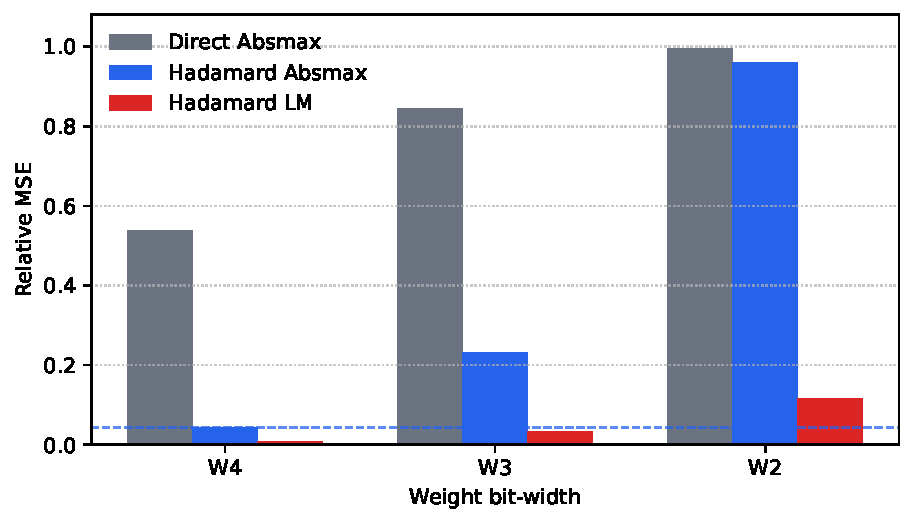
\includegraphics[width=0.82\linewidth]{image/stage_a_tensor_mse.pdf}
  \caption{A 线权重 relative MSE 对比}
  \label{fig:stage-a-tensor-mse}
\end{figure}

图~\ref{fig:stage-a-ppl} 给出 model-level PPL。Hadamard Absmax W4 的 PPL 为 15.40，明显优于 Direct Absmax W4，但 W3 和 W2 均发生崩溃。Hadamard LM W4 的 PPL 为 8.63，接近 FP16；Hadamard LM W3 的 PPL 为 12.99，优于 Hadamard Absmax W4，满足 A 线核心判断。Hadamard LM W2 的 tensor 指标仍明显好于 uniform 方法，但 PPL 已升至 19646.84，说明 W2 是当前失败边界。

\begin{figure}[!htbp]
  \centering
  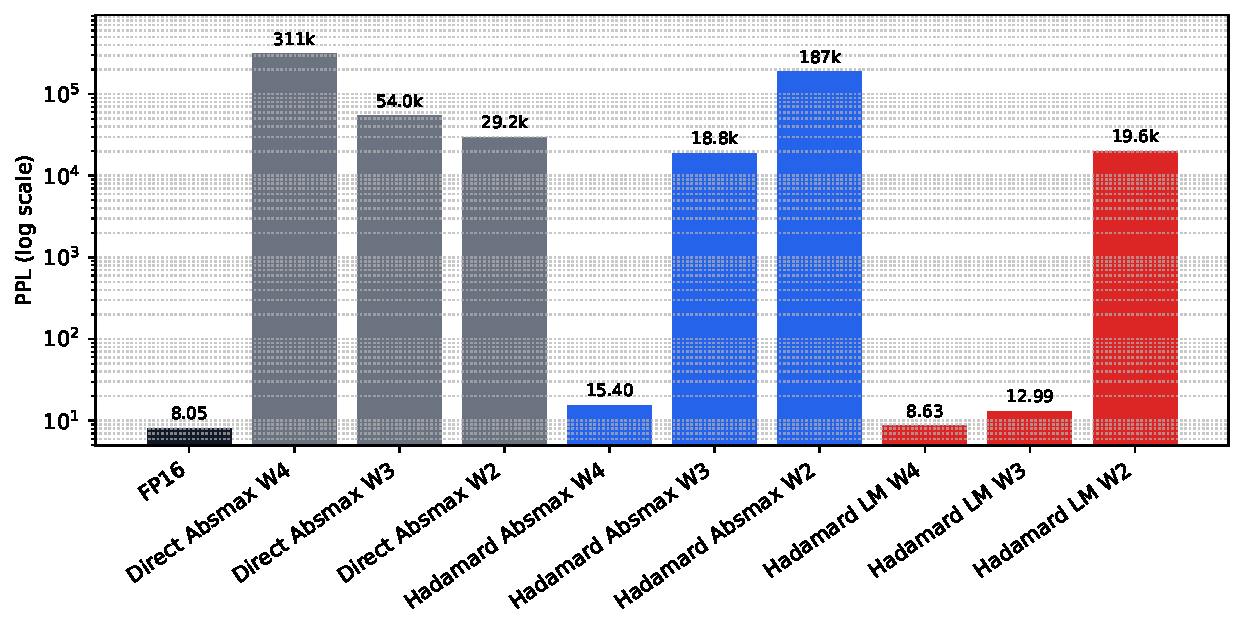
\includegraphics[width=0.88\linewidth]{image/stage_a_ppl.pdf}
  \caption{A 线 model-level PPL 对比；纵轴使用对数坐标}
  \label{fig:stage-a-ppl}
\end{figure}

综上，A 线得到三点发现。第一，Direct Absmax 在 TinyLlama weight-only 场景下不稳定，不能作为有效低比特主方法。第二，Hadamard Absmax 仅在 W4 上可用，W3/W2 在 model-level PPL 上崩溃。第三，Hadamard LM W3 的 PPL 优于 Hadamard Absmax W4，说明 Lloyd-Max 在旋转域中可以用非均匀 codebook 换取更低 weight bit；但 W2 暂时只能作为失败边界。

\subsection{B 线：FFN W/A Fake Quantization}

B 线实验回答的问题是：在 FFN 的 W/A fake quant 中，旋转域 Lloyd-Max 是否能使 W/A 位宽从 W4A4 推进到 W3A4 或 W4A3。实验按 activation tensor、local Linear/FFN output 和 FFN-only model-level PPL 三个层次展开，用于观察低一档 weight bit 或 activation bit 是否仍能保持数值质量。

实验比较 Direct-Absmax、Rot-Absmax 和 Rot-LM 三类方法。Activation tensor-level 实验覆盖 A4、A3 和 A2；local Linear/FFN 实验覆盖 Direct-Absmax W4A4、Rot-Absmax W4A4，以及 Rot-LM 的 W4A4、W3A4、W4A3、W3A3 和 W2A4；FFN-only PPL 实验比较 FP16、FFN Direct-Absmax W4A4、FFN Rot-Absmax W4A4，以及 FFN Rot-LM 的 W4A4、W3A4 和 W4A3。

图~\ref{fig:stage-b-activation-mse} 给出关键 activation site 上的 relative MSE 对比。除 \texttt{k\_proj\_out} 中 Rot-LM A3 略高于 Rot-Absmax A4 外，其余 site 上 Rot-LM A3 均低于 Rot-Absmax A4；在 \texttt{ffn\_intermediate} 上，二者差距尤为明显。这说明 activation 在旋转域中具备从 A4 推进到 A3 的数值空间。

\begin{figure}[!htbp]
  \centering
  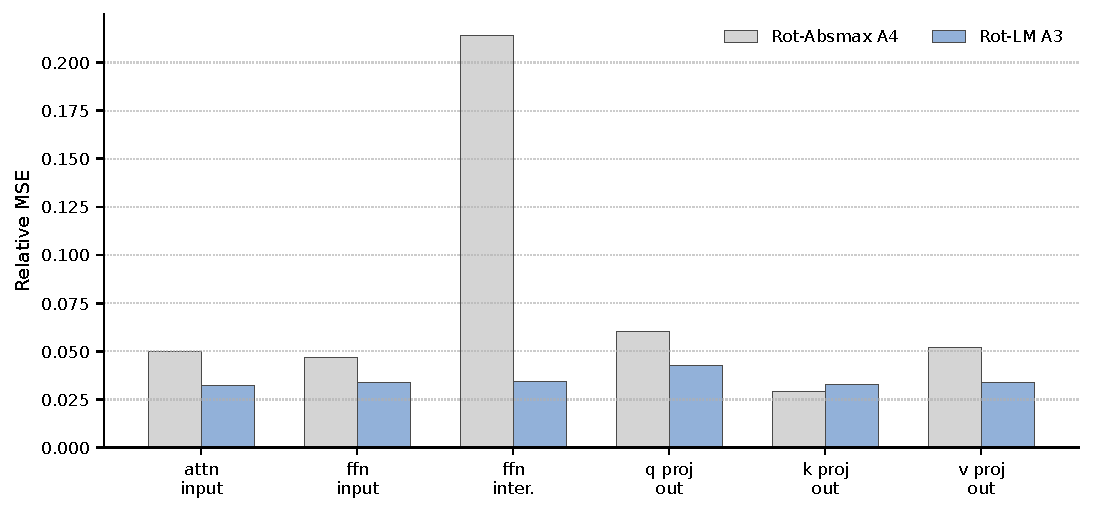
\includegraphics[width=0.86\linewidth]{image/stage_b_activation_mse.pdf}
  \caption{B 线 activation relative MSE 对比}
  \label{fig:stage-b-activation-mse}
\end{figure}

表~\ref{tab:stage-b-local} 汇总 local Linear 与完整 FFN output error。Direct-Absmax W4A4 与 Rot-Absmax W4A4 在 FFN 上均出现较高误差，而 Rot-LM 在 W4A4 下显著降低 local error。更重要的是，Rot-LM W3A4 与 Rot-LM W4A3 在 Linear 和 FFN 两个 scope 上都明显优于 Rot-Absmax W4A4，说明 weight bit 或 activation bit 单独降至 3 bit 后仍能保持较好的局部数值质量。

\begin{table}[!htbp]
  \centering
  \caption{B 线 local Linear/FFN output error 汇总}
  \label{tab:stage-b-local}
  \footnotesize
  \begin{tabular}{lllrrr}
    \toprule
    Scope & Method & Bits & Relative MSE & Cosine & SQNR dB \\
    \midrule
    Linear & Direct Absmax & W4A4 & 0.6133 & 0.6334 & 3.5532 \\
    Linear & Rot Absmax & W4A4 & 0.2286 & 0.9018 & 9.5292 \\
    Linear & Rot LM & W4A4 & 0.0159 & 0.9923 & 20.2219 \\
    Linear & Rot LM & W3A4 & 0.0372 & 0.9823 & 16.4159 \\
    Linear & Rot LM & W4A3 & 0.0374 & 0.9828 & 16.3506 \\
    Linear & Rot LM & W3A3 & 0.0582 & 0.9734 & 14.3239 \\
    FFN & Direct Absmax & W4A4 & 0.9700 & 0.2444 & 0.8008 \\
    FFN & Rot Absmax & W4A4 & 0.4775 & 0.8101 & 3.6001 \\
    FFN & Rot LM & W4A4 & 0.0312 & 0.9848 & 15.3302 \\
    FFN & Rot LM & W3A4 & 0.0731 & 0.9644 & 11.5625 \\
    FFN & Rot LM & W4A3 & 0.0792 & 0.9643 & 11.1068 \\
    FFN & Rot LM & W3A3 & 0.1212 & 0.9440 & 9.2538 \\
    \bottomrule
  \end{tabular}
\end{table}

图~\ref{fig:stage-b-ppl} 给出 FFN-only model-level PPL。FFN Direct-Absmax W4A4 与 FFN Rot-Absmax W4A4 分别升至 46090.42 和 2733.09，说明 uniform fake quant 在 FFN 结构中仍然不稳定。相比之下，FFN Rot-LM W4A4 的 PPL 为 8.59，接近 FP16；FFN Rot-LM W3A4 与 W4A3 的 PPL 分别为 9.98 和 9.35，均保持在较低水平，并显著优于 Rot-Absmax W4A4。

\begin{figure}[!htbp]
  \centering
  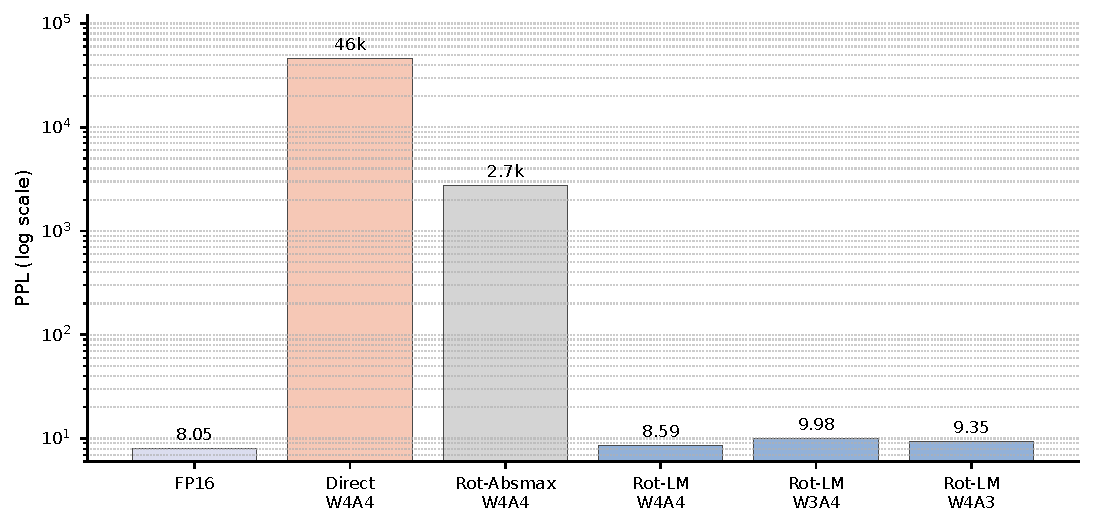
\includegraphics[width=0.88\linewidth]{image/stage_b_ppl.pdf}
  \caption{B 线 FFN-only model-level PPL 对比；纵轴使用对数坐标}
  \label{fig:stage-b-ppl}
\end{figure}

综上，B 线得到三点发现。第一，Rot-LM A3 平均优于 Rot-Absmax A4，说明 activation 旋转域中存在 A4 到 A3 的位宽下降空间。第二，Rot-LM W3A4 与 Rot-LM W4A3 在 Linear 和完整 FFN local output 上均显著优于 Rot-Absmax W4A4。第三，FFN-only PPL 与 local 结果一致，支持非均匀 codebook 换取更低 W/A 位宽的数值可行性。

\subsection{C 线：Attention/KV Cache 量化}

C 线实验回答的问题是：post-RoPE KV cache 的低比特量化是否能够保持 attention score 与 attention output，QJL residual 是否能进一步修正 Key quantization 的 inner-product 误差，以及 Attention 线性 W/A fake quant 与 KV cache low-bit quant 串联后，model-level PPL 是否仍可接受。实验依次考察 KV-local、QJL residual 和结构适配后的完整 Attention 层。

实验首先验证 post-RoPE Q/K 的 head-wise H64 rotation 在 no-quant 情形下保持 attention 计算不变性。随后，C2/C3 主要观察 score relative MSE、softmax KL、top-k overlap 和 output cosine；C4/C5 则采用 Attention 结构适配路径，将 Attention 线性层 W/A fake quant 与 KV cache 量化串联起来，分别评价整层输出误差与 Attention-only PPL。

表~\ref{tab:stage-c-kv-local} 汇总 C1 invariance 与 C2 KV-local 的关键结果。No-quant H64 rotation 的 score relative MSE 为 0，output cosine 为 1.0000，说明 post-RoPE Q/K 的 head-wise rotation 本身不破坏 attention score。进入 KV quantization 后，Hadamard-LM K4V4 明显优于 Absmax K4V4；Hadamard-LM K3V4 的 score relative MSE、softmax KL、top-k overlap 和 output cosine 也均略优于 Absmax K4V4，说明 Key 降至 3 bit 后仍具备局部可行性。Hadamard-LM K2V4 则明显退化，是当前失败边界。

\begin{table}[!htbp]
  \centering
  \caption{C 线 C1/C2 attention-local 指标汇总}
  \label{tab:stage-c-kv-local}
  \footnotesize
  \begin{tabular}{llrrrr}
    \toprule
    Method & KV Bits & Score MSE & Softmax KL & Top-k & Output Cosine \\
    \midrule
    H64 No-quant & K16V16 & 0.0000 & 0.0000 & 1.0000 & 1.0000 \\
    Absmax & K4V4 & 0.0127 & 0.2381 & 0.6884 & 0.9708 \\
    Hadamard-LM & K4V4 & 0.0031 & 0.0520 & 0.8183 & 0.9924 \\
    Hadamard-LM & K3V4 & 0.0116 & 0.1834 & 0.6902 & 0.9764 \\
    Hadamard-LM & K4V3 & 0.0031 & 0.0520 & 0.8183 & 0.9880 \\
    Hadamard-LM & K2V4 & 0.0421 & 0.5654 & 0.5343 & 0.9272 \\
    \bottomrule
  \end{tabular}
\end{table}

\begin{figure}[!htbp]
  \centering
  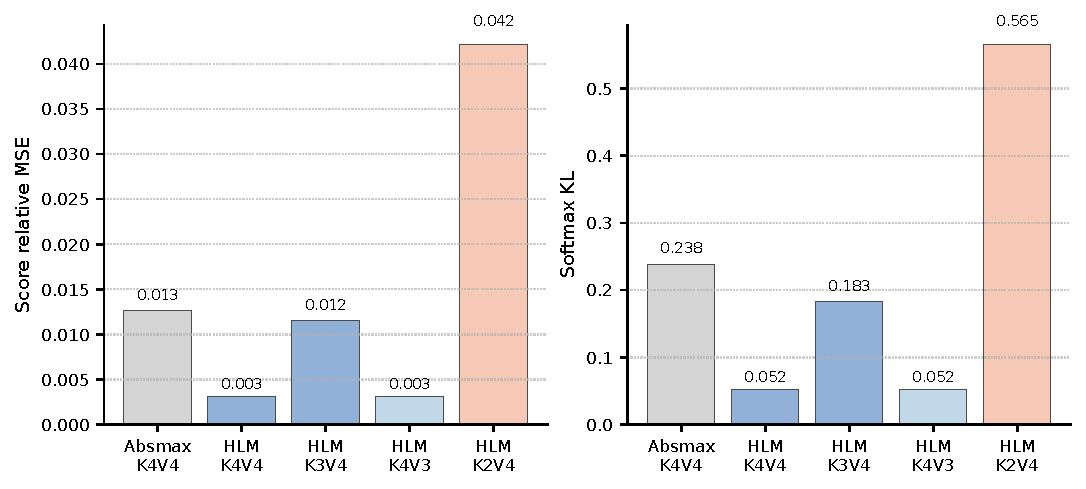
\includegraphics[width=0.88\linewidth]{image/stage_c_kv_local.pdf}
  \caption{C 线 KV-local score relative MSE 与 softmax KL 对比}
  \label{fig:stage-c-kv-local}
\end{figure}

表~\ref{tab:stage-c-qjl} 给出 QJL residual 结果。QJL correction 确实降低了部分 inner-product bias，例如 K3 base 的 bias 从 1.0115 降至 0.2042；但是 score relative MSE、softmax KL、top-k overlap 和 output cosine 均变差。K2 base 上也出现同样趋势。因此，当前 QJL residual 不进入 C5 默认实验组。

\begin{table}[!htbp]
  \centering
  \caption{C 线 C3 QJL residual 对比}
  \label{tab:stage-c-qjl}
  \footnotesize
  \begin{tabular}{lrrrr}
    \toprule
    Method & Score MSE & Softmax KL & Top-k & Output Cosine \\
    \midrule
    Hadamard-LM K2 & 0.0421 & 0.5654 & 0.5343 & 0.9272 \\
    Hadamard-LM K2 + QJL & 0.0595 & 0.9660 & 0.4917 & 0.8891 \\
    Hadamard-LM K3 & 0.0116 & 0.1834 & 0.6902 & 0.9764 \\
    Hadamard-LM K3 + QJL & 0.0176 & 0.2974 & 0.6452 & 0.9605 \\
    \bottomrule
  \end{tabular}
\end{table}

表~\ref{tab:stage-c-attention-local} 汇总结构适配后的 Attention-layer local 结果。Identity wrapper 的 layer output relative MSE 接近 0，说明 wrapper 本身不引入可见误差。KV-only K4V4 的 layer output cosine 为 0.9880；加入 Attention 线性 W/A fake quant 后，Rot-LM W4A4 + HLM K4V4 的 cosine 为 0.9569，仍保持较好局部质量。降位宽组合中，W4A3 + K4V3 优于 W3A4 + K3V4，表明 value/activation 降位宽在当前设置下比 weight/key 同时降位宽更稳。

\begin{table}[!htbp]
  \centering
  \caption{C 线 C4 structured Attention local output 汇总}
  \label{tab:stage-c-attention-local}
  \footnotesize
  \begin{tabular}{lllrr}
    \toprule
    Method & Linear Bits & KV Bits & Relative MSE & Cosine \\
    \midrule
    Attn Identity FP16 & FP16 & K16V16 & 0.0000 & 1.0000 \\
    Attn KV-HLM K4V4 & FP16 & K4V4 & 0.0246 & 0.9880 \\
    Attn KV-HLM K3V4 & FP16 & K3V4 & 0.0839 & 0.9618 \\
    Attn Rot-LM W4A4 + HLM K4V4 & W4A4 & K4V4 & 0.0891 & 0.9569 \\
    Attn Rot-LM W3A4 + HLM K3V4 & W3A4 & K3V4 & 0.2558 & 0.8817 \\
    Attn Rot-LM W4A3 + HLM K4V3 & W4A3 & K4V3 & 0.1623 & 0.9209 \\
    \bottomrule
  \end{tabular}
\end{table}

图~\ref{fig:stage-c-ppl} 给出 Attention-only model-level PPL。Attn Identity FP16 与 FP16 完全一致，说明完整替换路径保持基线行为。KV-only K4V4 和 K3V4 的 PPL 分别为 8.20 和 8.66，接近 FP16；structured Attention 中，Rot-LM W4A4 + HLM K4V4 的 PPL 为 8.61，仍在可接受范围内。Rot-LM W4A3 + HLM K4V3 的 PPL 为 9.39，而 Rot-LM W3A4 + HLM K3V4 升至 11.36，说明进一步降 weight/key 位宽会带来更明显的累积误差。

\begin{figure}[!htbp]
  \centering
  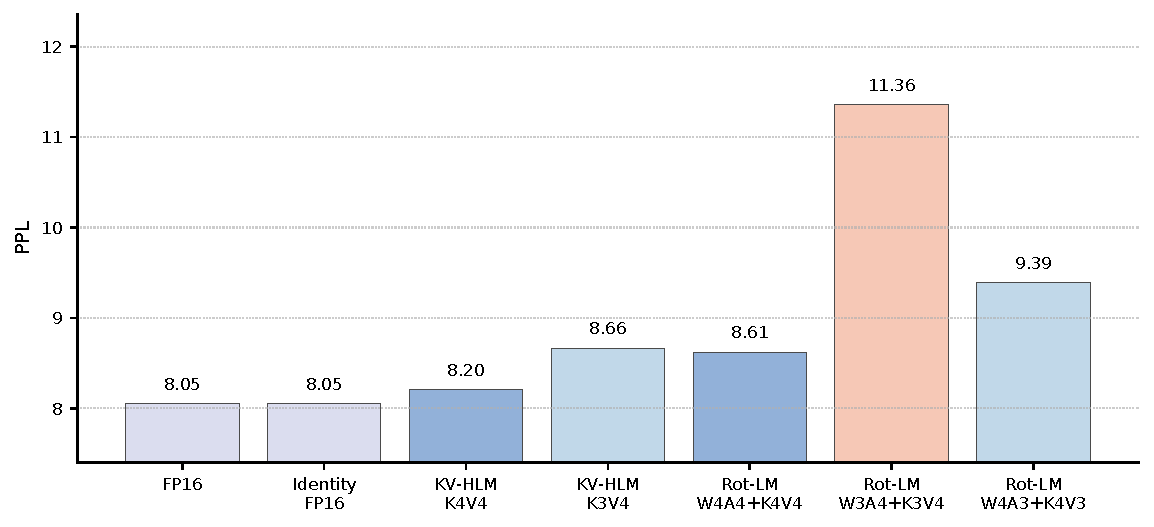
\includegraphics[width=0.90\linewidth]{image/stage_c_ppl.pdf}
  \caption{C 线 Attention-only model-level PPL 对比}
  \label{fig:stage-c-ppl}
\end{figure}

综上，C 线得到四点发现。第一，post-RoPE Q/K head-wise H64 rotation 在 no-quant 下保持 attention score 和 output。第二，Hadamard-LM K3V4 在 KV-local score、softmax 和 output 指标上具备可行性，K2V4 是失败边界。第三，当前 QJL residual 虽降低部分 inner-product bias，但整体 attention 指标变差，不适合作为默认方法。第四，Attention 结构适配后，local 指标与 model-level PPL 重新对齐；KV-only K4V4 和 structured W4A4 + K4V4 均接近 FP16，而 W3A4 + K3V4 仍可运行但误差更明显。

\section{实验结论}

当前实验的核心结论是：Hadamard rotation 与 Lloyd-Max codebook 在 TinyLlama 上能够显著改善低比特 fake quant 的数值质量，但其收益主要体现为位宽边界的推进。

A 线表明，Hadamard-LM W3 的 model-level PPL 优于 Hadamard Absmax W4，说明在 weight-only 场景中，旋转域非均匀量化可以把可用权重位宽从 4 bit 推向 3 bit；W2 虽有较好的 tensor reconstruction 指标，但 PPL 已经崩溃，暂时应视为失败边界。

B 线表明，FFN 中的 W/A fake quant 与 local output 指标具有较好一致性。Rot-LM W3A4 和 Rot-LM W4A3 在 Linear、完整 FFN 以及 FFN-only PPL 上均明显优于 Rot-Absmax W4A4，并且接近 FP16。这说明 FFN 是当前最稳定的低比特推进对象，activation 或 weight 单独降至 3 bit 具有明确数值可行性。

C 线表明，Attention/KV cache 对结构适配更敏感。post-RoPE Q/K head-wise H64 rotation 在 no-quant 下保持计算不变性；Hadamard-LM K3V4 在 KV-local 层面可行，K2V4 是失败边界；当前 QJL residual 未能改善整体 attention 指标。经过 Attention 结构适配后，KV-only K4V4 和 structured W4A4 + K4V4 的 PPL 接近 FP16，但 W3A4 + K3V4 的误差仍明显更大。

因此，当前实验最可靠的发现是：Hadamard rotation 负责削弱 outlier 并重塑分布，Lloyd-Max codebook 在旋转域中进一步降低低比特量化误差；二者结合能够在 weight-only、FFN W/A 和 KV-local 场景中给出 3 bit 可行性的算法证据。后续工作应集中在两点：一是将这些 fake quant 结果转化为可实现的 bit packing、codebook lookup 或专用 kernel；二是继续改进 Attention 结构量化，尤其是更稳健的 Key 低比特表示和 residual correction 方法。

\printbibliography[heading=bibintoc, title=\ebibname]

\end{document}
